\begin{frame}
\frametitle{What we want to introduce}
\begin{itemize}
\item How does a Constraint Model fit into a bigger system
\item Interaction with stakeholders
\item You define what the problem is
  \item 12 Steps to success
\end{itemize}
\end{frame}

\section{The Bigger Picture}

\begin{frame}
  \frametitle{CP Model is Part of a Larger System}
  \begin{itemize}
  \item Where do data come from?
  \item Control over data
  \item Generated plan
  \item Externalized representation of constraints
  \item Implementation of plan
    \item Feedback from previous runs
  \end{itemize}
\end{frame}


\begin{frame}
  \frametitle{Example: Datacenter Management}
  \begin{tikzpicture}[xscale=3,yscale=1.5,
       data/.style = {draw, rectangle,fill=green!20,align=center},
 result/.style = {draw, ellipse,fill=blue!20,align=center},
 program/.style = {draw,rectangle,rounded corners,fill=brown!20,align=center}]
    \node[data] (exo) at (1,3) {\shortstack{Electricity Price\\Weather Forecast}};
    \node[data] (vars) at (2,3) {\shortstack{Virtual\\Machines}};
    \node[data] (demand) at (3,3) {\shortstack{Demand\\Forecast}};
    \node[data] (current) at (1,2) {\shortstack{Current\\Assignment}};
    \node[program] (model) at (2,2) {\shortstack{VM\\Allocator}};
    \node[data] (constraints) at (3,2) {\shortstack{Resources}};
    \node[result] (plan) at (2,1) {VM Allocation};
    \node[program] (realization) at (2,0) {\shortstack{Management\\Platform}};
    \node[result] (actuals) at (2,-1) {\shortstack{Running VM}};
    \draw[->] (exo) -- (model);
    \draw[->] (vars) -- (model);
    \draw[->] (demand) -- (model);
    \draw[->] (current) -- (model);
    \draw[->] (constraints) -- (model);
    \draw[->] (model) -- (plan);
    \draw[->] (plan) -- (realization);
    \draw[->] (realization) -- (actuals);
    \draw[->] (actuals) -| (current);
  \end{tikzpicture}
  \end{frame}
    
\begin{frame}
  \frametitle{Example: Transport}
  \begin{tikzpicture}[xscale=3,yscale=1.5,
       data/.style = {draw, rectangle,fill=green!20,align=center},
 result/.style = {draw, ellipse,fill=blue!20,align=center},
 program/.style = {draw,rectangle,rounded corners,fill=brown!20,align=center},
 person/.style = {draw,rectangle,rounded corners,fill=red!20,align=center}]
    \node[data] (exo) at (1,3) {\shortstack{Expected\\Travel Times}};
    \node[data] (vars) at (2,3) {\shortstack{Transport\\Requests}};
    \node[data] (current) at (1,2) {\shortstack{Current\\Location}};
    \node[program] (model) at (2,2) {\shortstack{Transport\\Solver}};
    \node[data] (constraints) at (3,2) {\shortstack{Work Rules\\Preferences}};
    \node[result] (plan) at (2,1) {Planned Tours};
    \node[program] (realization) at (2,0) {\shortstack{Fleet\\Operation}};
    \node[result] (actuals) at (2,-1) {\shortstack{Actual Tours}};
    \node[person] (customer) at (3,3) {Customers};
    \node[person] (manager) at (4,2) {Manager};
    \node[person] (agents) at (4,0) {Agents};
    \draw[->] (exo) -- (model);
    \draw[->] (vars) -- (model);
    \draw[->] (current) -- (model);
    \draw[->] (constraints) -- (model);
    \draw[->] (model) -- (plan);
    \draw[->] (plan) -- (realization);
    \draw[->] (realization) -- (actuals);
    \draw[->] (actuals) -| (current);
    \draw[->] (customer) -- (vars);
    \draw[->] (manager) -- (constraints);
    \draw[->] (plan) -- (agents);
    \draw[->] (agents) -- (actuals);
    \draw[->] (agents) -- (manager);
    
  \end{tikzpicture}
  \end{frame}
    
\begin{frame}
  \frametitle{Example: Personnel Rostering}
  \begin{tikzpicture}[xscale=3,yscale=1.5,
       data/.style = {draw, rectangle,fill=green!20,align=center},
 result/.style = {draw, ellipse,fill=blue!20,align=center},
 program/.style = {draw,rectangle,rounded corners,fill=brown!20,align=center},
 person/.style = {draw,rectangle,rounded corners,fill=red!20,align=center}]
    \node[data] (exo) at (1,3) {\shortstack{Unplanned\\Unavailability\\Emergencies}};
    \node[data] (vars) at (2,3) {\shortstack{Demand\\Plan}};
    \node[data] (current) at (1,2) {\shortstack{History}};
    \node[program] (model) at (2,2) {\shortstack{Rostering\\Solver}};
    \node[data] (constraints) at (3,2) {\shortstack{Work Rules\\Preferences}};
    \node[result] (plan) at (2,1) {Planned Schedule};
    \node[program] (realization) at (2,0) {\shortstack{Operations}};
    \node[result] (actuals) at (2,-1) {\shortstack{Actual Schedule}};
    \node[person] (manager) at (4,3) {Manager};
    \node[person] (agents) at (4,0) {Staff};
    \draw[->] (exo) -- (model);
    \draw[->] (vars) -- (model);
    \draw[->] (current) -- (model);
    \draw[->] (constraints) -- (model);
    \draw[->] (model) -- (plan);
    \draw[->] (plan) -- (realization);
    \draw[->] (realization) -- (actuals);
    \draw[->] (actuals) -| (current);
    \draw[->] (manager) -- (vars);
    \draw[->] (manager) -- (constraints);
    \draw[->] (plan) -- (agents);
    \draw[->] (agents) -- (actuals);
    \draw[->] (agents) -- (manager);
    
  \end{tikzpicture}
  \end{frame}
    
\begin{frame}
  \frametitle{The General Scheme}
  \begin{tikzpicture}[xscale=3,yscale=1.5,
       data/.style = {draw, rectangle,fill=green!20,align=center},
 result/.style = {draw, ellipse,fill=blue!20,align=center},
 program/.style = {draw,rectangle,rounded corners,fill=brown!20,align=center}]
    \node[data] (exo) at (1,3) {\shortstack{Exogenous\\Data}};
    \node[data] (vars) at (2,3) {\shortstack{Decision\\Variables}};
    \node[data] (current) at (1,2) {\shortstack{Current\\State}};
    \node[program] (model) at (2,2) {\shortstack{Constraint\\Model}};
    \node[data] (constraints) at (3,2) {\shortstack{Constraints\\Preferences\\Objectives}};
    \node[result] (plan) at (2,1) {Plan};
    \node[program] (realization) at (2,0) {\shortstack{Realization}};
    \node[result] (actuals) at (2,-1) {\shortstack{Actuals}};
    \draw[->] (exo) -- (model);
    \draw[->] (vars) -- (model);
    \draw[->] (current) -- (model);
    \draw[->] (constraints) -- (model);
    \draw[->] (model) -- (plan);
    \draw[->] (plan) -- (realization);
    \draw[->] (realization) -- (actuals);
    \draw[->] (actuals) -| (current);
  \end{tikzpicture}
  \end{frame}

\begin{frame}
  \frametitle{Key Questions: How? Who? When? Where?}
  \begin{itemize}
  \item (How is work done?)
  \item Who performs work?
  \item When is it performed?
    \item (Where is it performed?)
  \end{itemize}
\end{frame}

\section{12 Steps to Success}

\begin{frame}
\frametitle{Step 1: Literature Review}
\begin{itemize}
\item Which problem are other people solving?
  \item What are the favourite tecniques, why?
  \item What tools are used?
    \item Learn the domain specific language
\end{itemize}
\end{frame}

\begin{frame}
\frametitle{Step 2: Description of Problem}
\begin{itemize}
\item Clearly defined use cases, ranked by importance
\item Textual description of problem before math
\item Important: Involve all stakeholders
\item Important: Identify champions and their benefits
  \item State what is outside the scope
\end{itemize}
\end{frame}

\begin{frame}
\frametitle{Step 3: Example Data and Solution}
\begin{itemize}
\item Best is years of existing data and solutions
\item Important: Set with manageable problem size
\item Independent checker of solutions
  \item Possible: Trivial problem example for manual exploration
\end{itemize}
\end{frame}

\begin{frame}
\frametitle{Step 4: Visualizing Results}
\begin{itemize}
\item Develop before solver
\item Visualize existing solutions
\item Perhaps end-users have existing visualizations
\item Generic views for classes of problems (global constraints)
  \item Helps to understand poor performance
  \item Also: Compute KPI (Key Performance Indicators)
\end{itemize}
\end{frame}

\begin{frame}
  \frametitle{Example Dashboard: Patient Waitlists}
  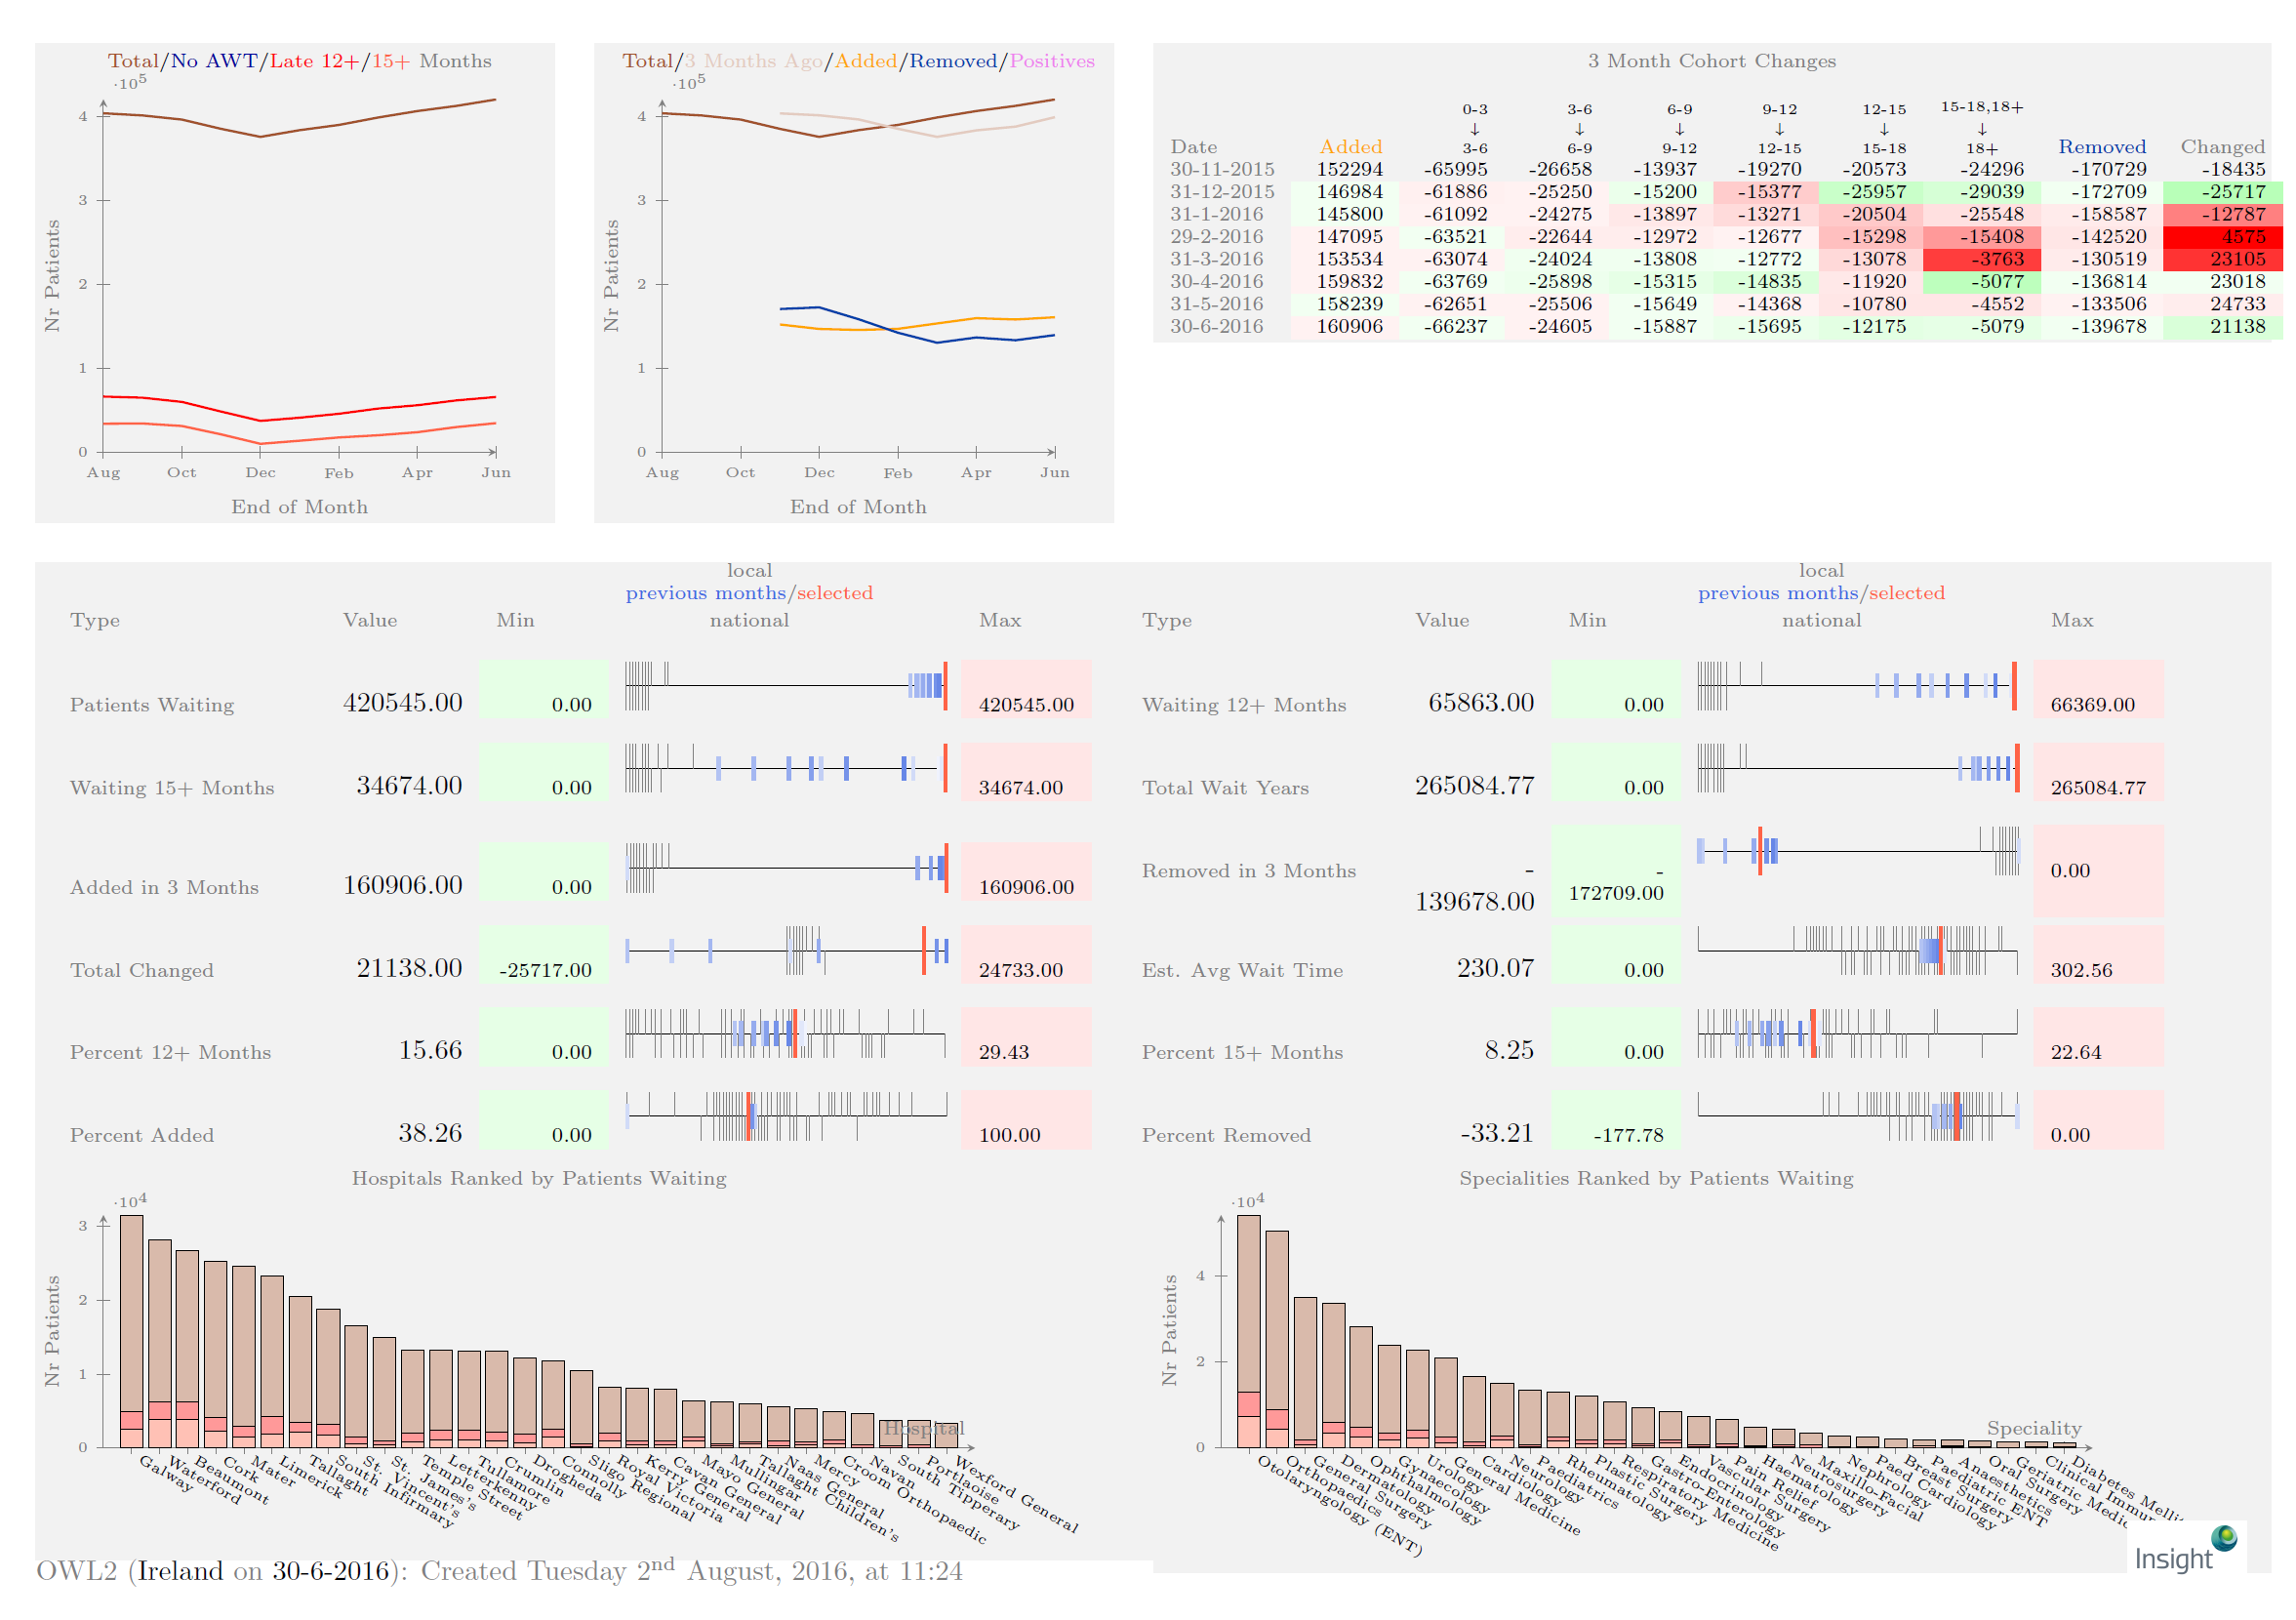
\includegraphics[width=10cm]{../methodology/images/ntpf}
  \end{frame}

\begin{frame}
\frametitle{Step 5: Implement Core Model}
\begin{itemize}
\item One constraint type at a time
\item Start with finding feasible, good solutions
\item Find lower/upper bounds to estimate solution quality
  \item Start with basic search strategy
\end{itemize}
\end{frame}

\begin{frame}
\frametitle{Step 6: Feedback from Domain Experts}
\begin{itemize}
\item Are you solving the right problem?
  \item Are all stakeholders happy with solution and objectives?
\end{itemize}
\end{frame}

\begin{frame}
\frametitle{Step 7: Study Obvious Alternatives}
\begin{itemize}
\item If you have time (PhD students have time)
\item Is there a straight-forward MIP/SAT model of problem?
\item Do they work on small scale, large scale problems?
\item Can you come up with good, feasible heuristics?
\end{itemize}
\end{frame}

\begin{frame}
\frametitle{Step 8: Solve Integration Issues}
\begin{itemize}
\item Not too early, time wasted if solver does not work
\item Not too late, without integration solver is just a demonstrator
\end{itemize}
\end{frame}

\begin{frame}
\frametitle{Step 9: Performance Engineering}
\begin{itemize}
\item Problem specific search strategies
\item Parallelism
\item Improved model
\item Improved solver
  \item Parameter tuning
\end{itemize}
\end{frame}

\begin{frame}
\frametitle{Step 10: Fight Feature Creep}
\begin{itemize}
\item If it works, then people want more
\item Not in first release
\item Implement core use case, nothing more
  \item Exception: Allow all constraints to be optional
\end{itemize}
\end{frame}

\begin{frame}
\frametitle{Step 11: Improve Stability}
\begin{itemize}
  \item What is really required?
  \item Remove experimental code
  \item How far can we push model?
  \item Code review against model description
    \begin{itemize}
      \item Allow changes in description
    
\end{itemize}
\end{itemize}
\end{frame}

\begin{frame}
\frametitle{Step 12: Tell the World}
\begin{itemize}
\item Dozens of good CP applications hidden from view
\item Consider writing application paper
  \begin{itemize}
    \item Involve end-users and stakeholders
    \item Describe problem from their perspective
    \item If possible, publish data set and constraint description      
  \end{itemize}
\item Submit instances to solver competitions
  \begin{itemize}
    \item Other people will work on improved performance of your model
\end{itemize}
\end{itemize}
\end{frame}

\section{Constraints in an Uncertain World}

\begin{frame}
  \frametitle{The ICON Loop}
  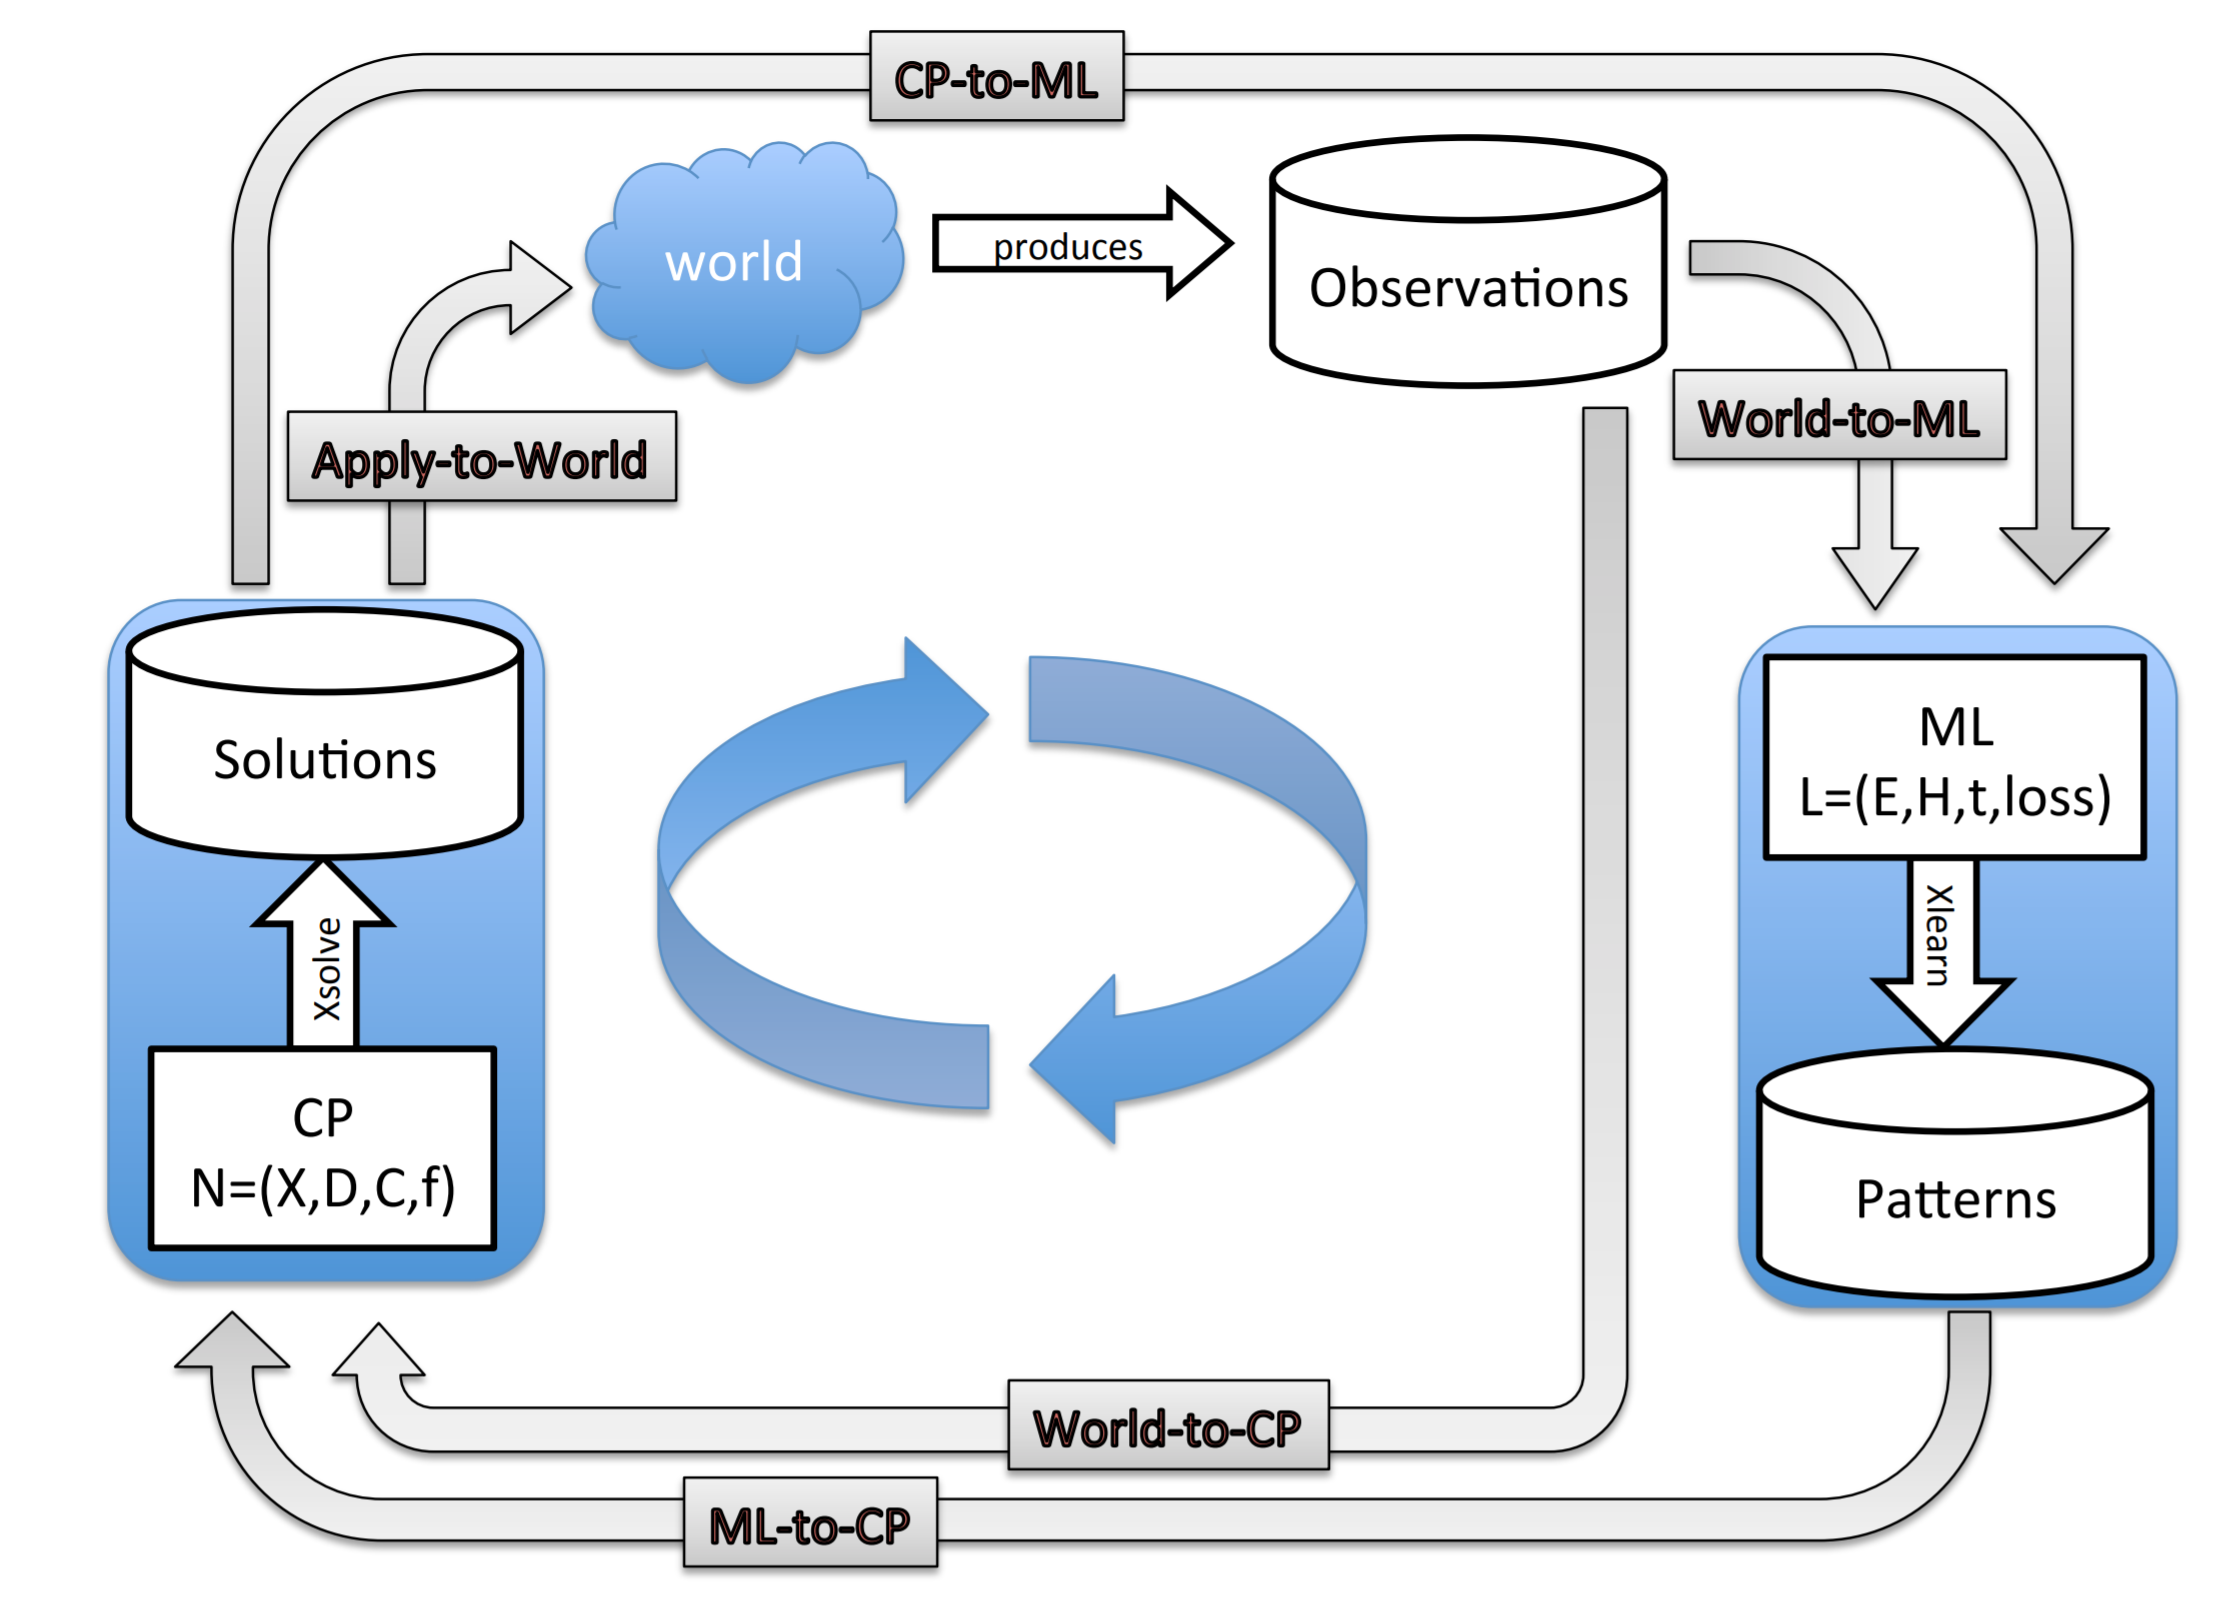
\includegraphics[width=10cm]{../methodology/images/iconloop}
\end{frame}

\begin{frame}
  \frametitle{A Blueprint for Interaction}
  \begin{itemize}
  \item Developed in the European ICON project
  \item Partners KU Leuven, Montpellier, Pisa, UCC
    \item Ways of combining Machine Learning with CP
  \end{itemize}
\end{frame}

\begin{frame}
  \frametitle{Example: Intra-City Transport}
  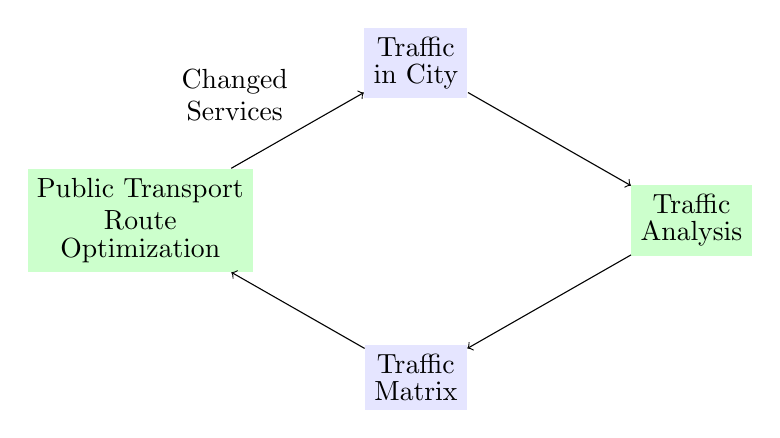
\begin{tikzpicture}[xscale=3.5,yscale=2]
    \node[fill=blue!10] (World) at (2,2) {\shortstack{Traffic\\in City}};
    \node[fill=green!20] (ML) at (3,1) {\shortstack{Traffic\\Analysis}};
    \node[fill=blue!10] (Forecast) at (2,0) {\shortstack{Traffic\\Matrix}};
    \node[fill=green!20] (CP) at (1,1) {\shortstack{Public Transport\\Route\\Optimization}};
    \draw[->] (World) -- (ML);
    \draw[->] (ML) -- (Forecast);
    \draw[->] (Forecast) -- (CP);
    \draw[->] (CP) -- node[above left] {\shortstack{Changed\\Services}} (World);
  \end{tikzpicture}
  \noindent\begin{itemize}
  \item Optimization only as good as data feeding into it
    \end{itemize}
\end{frame}

\begin{frame}
  \frametitle{Feedback May Lead to More Traffic}
  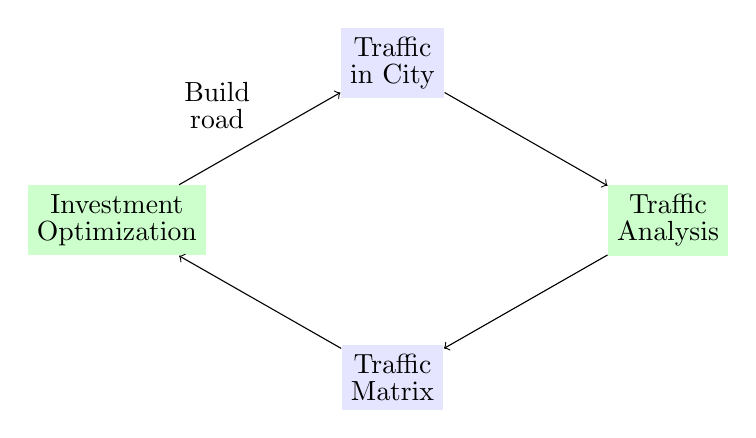
\begin{tikzpicture}[xscale=3.5,yscale=2]
    \node[fill=blue!10] (World) at (2,2) {\shortstack{Traffic\\in City}};
    \node[fill=green!20] (ML) at (3,1) {\shortstack{Traffic\\Analysis}};
    \node[fill=blue!10] (Forecast) at (2,0) {\shortstack{Traffic\\Matrix}};
    \node[fill=green!20] (CP) at (1,1) {\shortstack{Investment\\Optimization}};
    \draw[->] (World) -- (ML);
    \draw[->] (ML) -- (Forecast);
    \draw[->] (Forecast) -- (CP);
    \draw[->] (CP) -- node[above left] {\shortstack{Build\\road}} (World);
  \end{tikzpicture}
  \noindent\begin{itemize}
  \item The ``world'' reacts to changes
  \item That may be difficult to predict
    \end{itemize}
\end{frame}

\begin{frame}
  \frametitle{Reacting to Real-time Electricity Prices}
  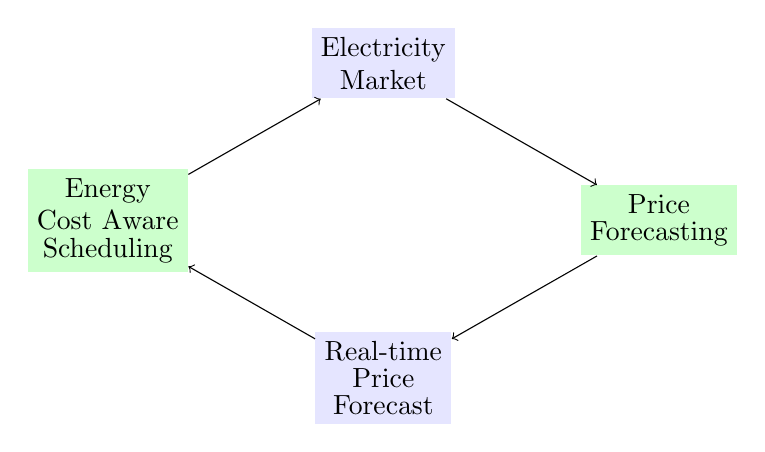
\begin{tikzpicture}[xscale=3.5,yscale=2]
    \node[fill=blue!10] (World) at (2,2) {\shortstack{Electricity\\Market}};
    \node[fill=green!20] (ML) at (3,1) {\shortstack{Price\\Forecasting}};
    \node[fill=blue!10] (Forecast) at (2,0) {\shortstack{Real-time\\Price\\Forecast}};
    \node[fill=green!20] (CP) at (1,1) {\shortstack{Energy\\Cost Aware\\Scheduling}};
    \draw[->] (World) -- (ML);
    \draw[->] (ML) -- (Forecast);
    \draw[->] (Forecast) -- (CP);
    \draw[->] (CP) --  (World);
  \end{tikzpicture}
  
  \noindent\begin{itemize}
  \item Good way to optimize cost individually
  \item May lead to oscillation if everybody does it
    \end{itemize}
\end{frame}



\section{There is no ``The Model''}

\begin{frame}[fragile]
  \frametitle{Feedback Loops in Modelling}
  \scalebox{0.5}{
\begin{tikzpicture}[node distance=10mm,
 block/.style = {draw, rectangle,fill=green!20,align=center},
 human/.style = {draw, ellipse,fill=blue!20,align=center},
 software/.style = {draw,rectangle,rounded corners,fill=brown!20,align=center},
                        ]
  \node[cloud,draw,fill=red!10] (problem) at (2,10) {Problem};
  \node[human,below=of problem] (user) {User};
  \node[block,below=of user] (description) {\shortstack{(Informal)\\Description}};
  \node[human,below=of description] (modeler) {Modeler};
  \node[block,below=of modeler] (model) {Model};
  \node[software,below=of model] (solver)  {Solver};
  \node[block,below=of solver] (solution)  {\shortstack{Proposed\\Solution}};
  \node[human,right=2cm of solver] (designer)  {Designer};
  \node[software,left=2.5cm of model] (integration)  {Integration};
  \node[block,above=of designer] (bias) {\shortstack{Constraint\\Bias}};
  \draw[->] (problem) -- (user);
  \draw[->] (user) -- (description);
  \draw[->] (description) -- (modeler);
  \draw[->] (modeler) -- (model);
  \draw[->] (model) -- (solver);
  \draw[->] (solver) -- (solution);
  \draw[->] (designer) -- (solver);
  \draw[<->] (bias) |- (modeler);
  \draw[<->] (bias) -- (designer);
  \draw[->] (solution.east) -| (designer.south);
  \draw[->] (solution.west) -- ++(-1,0) |- (modeler.west);
  \draw[->] (solution.west) -- ++(-2,0) |- (user.west);
  \draw[->] (solution.west) -| (integration.south);
  \draw[->] (integration.north) |- (problem.west);
\end{tikzpicture}
}
\end{frame}

\begin{frame}[fragile]
  \frametitle{The Future: Automated Modelling}
  \scalebox{0.45}{
    \begin{tikzpicture}[node distance=10mm,
 block/.style = {draw, rectangle,fill=green!20,align=center},
 human/.style = {draw, ellipse,fill=blue!20,align=center},
 software/.style = {draw,rectangle,rounded corners,fill=brown!20,align=center},
                        ]
  \node[cloud,draw,fill=red!10] (problem) at (2,10) {Problem};
  \node[block,below=of problem] (samples) {\shortstack{Sample/Historical\\Solutions}};
  \node[software,below=of samples] (modelseeker)  {ModelSeeker};
  \node[block,below=of modelseeker] (elements) {\shortstack{Model\\Elements}};
  \node[human,below=of elements] (modeler) {User/Modeler};
  \node[block,below=of modeler] (model) {Model};
  \node[software,below=of model] (solver)  {Solver};
  \node[block,below=of solver] (solution)  {\shortstack{Proposed\\Solution}};
  \node[software,right=2cm of solver] (generator)  {\shortstack{Solver\\Generator}};
  \node[software,left=2.5cm of model] (integration)  {Integration};
  \node[block,above=of generator] (bias) {\shortstack{Constraint\\Bias}};
  \draw[->] (problem) -- (samples);
  \draw[->] (samples) -- (modelseeker);
  \draw[->] (modelseeker) -- (elements);
  \draw[->] (elements) -- (modeler);
  \draw[->] (modeler) -- (model);
  \draw[->] (model) -- (solver);
  \draw[->] (solver) -- (solution);
  \draw[->] (generator) -- (solver);
  \draw[<->] (bias) |- (modelseeker);
  \draw[->] (bias) -- (generator);
  \draw[->] (solution.east) -| (generator.south);
  \draw[->] (solution.west) -- ++(-1.5,0) |- (modeler.west);
  \draw[->] (solution.west) -| (integration.south);
  \draw[->] (integration.north) |- (problem.west);
\end{tikzpicture}

  }
\end{frame}



\section{Conclusion}

\begin{frame}
\frametitle{Points to Remember}
\begin{itemize}
\item A CP application is part of a larger system
\item CP Model is rarely cause of project failure
  \begin{itemize}
  \item No clear champion
  \item No clear use case
  \item Data not available/data quality    
  \end{itemize}
\item Every problem is different, you decide what to model
  \item Understand the interaction between tools and problem
\end{itemize}
\end{frame}

